\chapter{Problem with the Concurrent Analysis Method}

The analysis technique presented in the previous chapter, propagates the data flow values across inter-thread edges in the same way as it propagates the data flow flow along inter-thread edges. Consider the output of heap-liveness analysis technique on the same example of the previous chapter. The figure 5.1 is the final data flow value obtained after convergence. \\

\begin{figure}
	\centering
	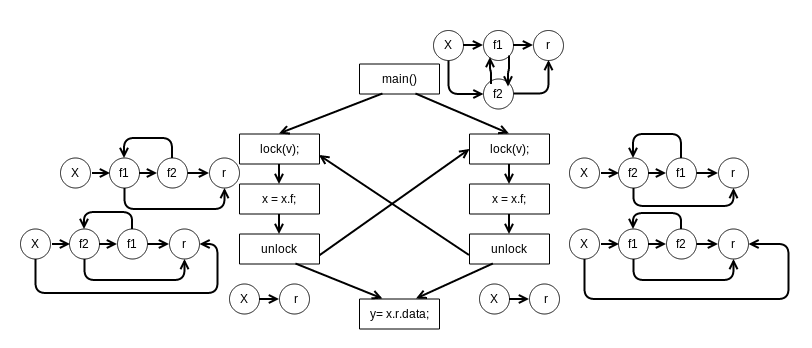
\includegraphics[width=0.8\textwidth]{Figures/conc_analysis_itr4.png}
	\caption{Example of the concurrent analysis technique}
	\label{fig:ch5example}
\end{figure}


At the program point containing the main statement, the possible live links would be \emph{x.f1.f2.r} or \emph{x.f2.f1.r}. However the final data flow value  obtained at the main statement includes access links \emph{x.f1.r}, \emph{x.f2.r} , \emph {x.\{f2.f1\}\textsuperscript{+}.r}, \emph{x.\{f1.f2\}\textsuperscript{+}.r} which are imprecise values. The major source of error is due to the transitions from node $f_1$ to $f_2$ and from $f_2$ to $f_1$ in the access graph. \\

The imprecise data flow values are a result of taking into account execution of critical sections more than once. The thread synchronization edges introduce loops in the program graph. The current method treats these thread synchronization edges as loops and continues propagation of the facts until a converged value is obtained (as seen in the previous chapter). \\

\section{Execution of Critical Sections}

The execution of a multi-threaded program is an interleaving of statements of the multiple threads. Critical sections are regions where the shared variables are  Thus there is a need to identify the critical sections that only execute once. The analysis to figure this out is thread independent. Note that a critical section can only be executed once if there are no backward program edges from a statement after unlock(v) to one before lock(v). For such critical sections we need to keep track to thread switches encountered while performing the analysis. In the example figure 5.1, if the critical section of thread 1 is analyzed and the data flow value is transferred to thread 2 for analysis along an inter-thread edge, it is required to ensure that data flow value in not transferred back to thread 1 after analysis of thread 2 critical section. \\

For handling such cases, we need to examine the presence of loops within each thread. 
\begin{itemize}
	\item If there is no loop within and across a critical section, it can only be executed once.
	\item If a loop is present within a critical section, even then the critical section can be executed only once. This is so because if 1 thread enters a critical section, all other threads wait until the this thread completes executing the loop inside the critical section.
	\item It a loop is present across a critical section in a thread, then the critical section can 
\end{itemize}
          